\newcommand{\texCommand}[1]{\texttt{\textbackslash{#1}}}%

\newcommand{\exemplo}[1]{%
\vspace{\baselineskip}%
\noindent\fbox{\begin{minipage}{\textwidth}#1\end{minipage}}%
\\\vspace{\baselineskip}}%

\newcommand{\exemploVerbatim}[1]{%
\vspace{\baselineskip}%
\noindent\fbox{\begin{minipage}{\textwidth}%
#1\end{minipage}}%
\\\vspace{\baselineskip}}%


Este capítulo busca elucidar conceitos importantes para o entendimento do trabalho, partindo de uma melhor descrição da COVID-19 iniciada na introdução, assim como suas politicas publicas e o dessas impacto em diversas regiões. Bem como uma conceitos essenciais sobre modelagem espacialmente explícitas utilizando-se software de modelagem multiagente. Seguindo a partir disso apresentar no capitulo 2.1...

%%%%%%%%%%%%%%%%%%%%%%%%%%%%%%%%%%%%%%%%%%%%%%%%%%%%%%%%%%%%%%%%%%%%%%%%%%%%%%%%
%%%%%%%%%%%%%%%%%%%%%%%%%%%%%%%%%%%%%%%%%%%%%%%%%%%%%%%%%%%%%%%%%%%%%%%%%%%%%%%%
%%%%%%%%%%%%%%%%%%%%%%%%%%%%%%%%%%%%%%%%%%%%%%%%%%%%%%%%%%%%%%%%%%%%%%%%%%%%%%%%
\section{A Pandemia da COVID-19}

A Organização Pan-Americana da Saúde (OPAS) publicou que em 31 de dezembro de 2019, a Organização Mundial da Saúde (OMS) foi alertada sobre casos de pneumonia na cidade de Wuhan, província de Hubei, na República Popular da China. A nova cepa, até o momento ainda desconhecida a seres humanos de coronavírus foi confirmada em janeiro de 2020.

Ao todo, sete coronavírus humanos (HCoVs) já foram identificados: HCoV-229E, HCoV-OC43, HCoV-NL63, HCoV-HKU1, SARS-COV (que causa síndrome respiratória aguda grave), MERS-COV (que causa síndrome respiratória do Oriente Médio) e o, mais recente, novo coronavírus (que no início foi temporariamente nomeado 2019-nCoV e, em 11 de fevereiro de 2020, recebeu o nome de SARS-CoV-2). Esse novo coronavírus é responsável por causar a doença COVID-19.

No Brasil, foi inicialmente declarado uma Emergência de Saúde Pública de Importância Nacional (ESPIN) de acordo com a Portaria Nº 188, de 3 de fevereiro de 2020 publicada no Diário Oficial da União, a portaria recomendou divulgar informações a população e até o momento não aplicou determinações restritivas para controle da COVID-19, chamada até a data da divulgação da portaria de  2019-nCoV.

De acordo com informações divulgadas pela Organização Pan-Americana da Saúde (OPAS), foi declarado em 11 de março de 2020 com objetivo de interromper a propagação do vírus uma Emergência de Saúde Pública de Importância Internacional (ESPII) – o mais alto nível de alerta da Organização.  


\section{O que são coronavírus}

Os coronavírus são uma família de vírus que possuem esse nome por conta das espículas na sua superfície que assemelham a uma coroa. Alguns sintomas vão desde resfriado leve, a síndrome respiratória aguda grave. Essa família começou a ser estudada em meados de 1960,  porém foi observado maior foco nesses vírus a partir de 2002 com o SARS (SARS-CoV), no qual essa nova variante era mais mortal e contagiosa do que as anteriores. 

\section{Tipos de coronavírus}

Atualmente são conhecidos 7 tipos de coronavirus que podem causar infecções respiratórias:

\begin{itemize}
\item Alfa coronavirus 229E e NL63;
\item Beta coronavirus OC43 e HKU1;
\item SARS-CoV;
\item MERS-CoV;
\item SARS-CoV-2.
\end{itemize}

\section{Impacto dos coronavírus }

Desses vírus já citados tanto os Alfa coronavirus quanto os Beta coronavirus já estavam presente no sociedade, porém seu impacto não é visto de forma tão alarmantes, pois seus sintomas estão associados a gripes comuns e problemas gastrointestinais como diarreias, náuseas e vômitos.

SARS-CoV (causador da Síndrome Respiratória Aguda Grave ou SARS), segundo a Organização Mundial da Saúde(OMS) foi a primeira nova doença grave e prontamente transmissível a surgir no século 21 e mostrou uma clara capacidade de se espalhar pelas rotas das viagens aéreas internacionais. O impacto dessa cepa foi notado ainda final de 2002 se espalhando por mais de 26 países e contaminando mais de 8000 pessoas até que foi totalmente controlada em julho de 2003, a Organização Mundial da Saúde definiu sua letalidade em torno de 3\%.

MERS-CoV (causador da Síndrome Respiratória do Oriente Médio ou MERS) gerou uma visibilidade internacional após em um surto em abril de 2012 na Arabia Saudita e diferente da SARS-CoV que foi controlada em menos de 1 ano, o MERS-CoV, segundo a Organização Mundial da Saúde, somente foi erradicado em fevereiro de 2022. Como pode ser observado na imagem abaixo.

O Novo Coronavirus inicialmente conhecido como 2019-nCoV começou a se propagar em Wuhan, na China no final de 2019 que posteriormente se espalhou pelo mundo, atingindo mais de 120 países (Ribeiro & Silva, 2021).

O nome da doença foi posteriormente sugerido como COVID-19 pela Organização Mundial da Saúde(OMS). Algum tempo depois o Comitê Internacional de Taxonomia de Vírus denominou o vírus como SARS-CoV-2.

Segundo o Ministério da Saúde, o Brasil já ultrapassou os 30 milhões de pessoas que foram infectados desses mais de 29 milhões recuperados e mais de 660 mil óbitos. Além disso segundo a Organização Mundial da Saúde o número de infectados já ultrapassava 511 milhões de pessoas.

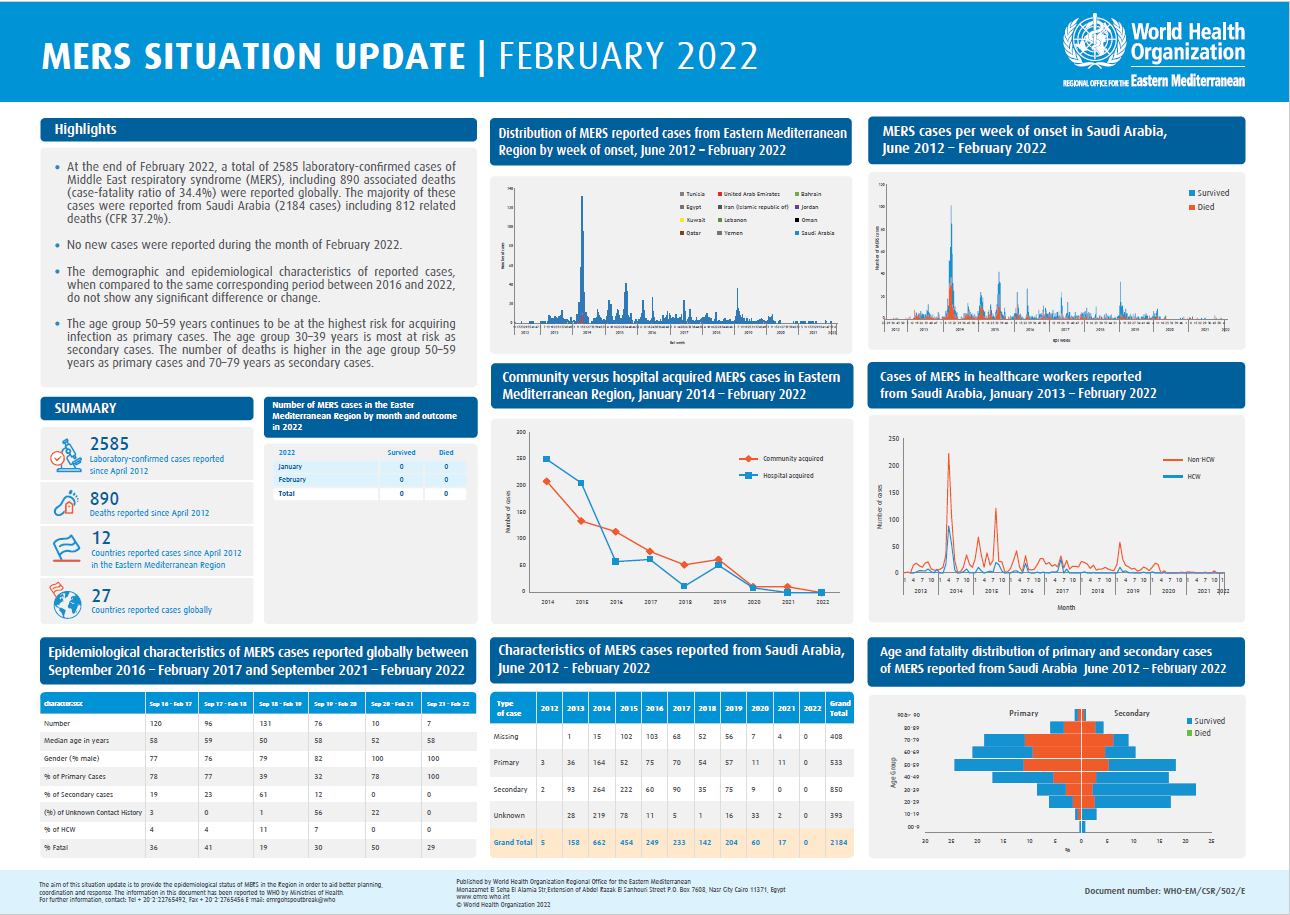
\includegraphics[width=16cm, height=16cm]{MERS.PNG}

\section{Epidemiologia do COVID-19}

O COVID-19 possui características muito semelhantes ao do SARS-CoV, fato que é observado no trabalho de Zhou e colaboradores (2020) ao comparar o COVID-19 com coronavirus de encontrados em morcegos foi possível encontrar uma relação de 96\% de proximidade entre eles. Por conta disso suspeita-se que teve origem em morcegos passando posteriormente a algum animal intermediário que após sofrer mutações foi possível a transmissão para humanos(Nogueira e Silva, 2020), embora haja essas suspeitas ainda não foi encontrado esse animal intermediário. 

A propagação do COVID-19 já era especulado que seria também por gotículas presentes na fala, em tosses e espirros, contato pessoal próximo, como toque, abraço ou aperto de mão; contato com objetos ou superfícies contaminadas, seguido de contato com a boca, nariz ou olhos características que os outros coronavirus possuem na sua transmissão. Entretanto sua propagação é muito superior aos outros da sua família. Além disso, segundo a Organização Mundial da Saúde (OMS) embora o período de incubação do SARS-CoV possa ser de 2-10 dias, o do COVID-19 pode variar entre 5-12 dias, pode ser um agravante adicional para a propagação do vírus, pois como foi observado Zhengdong e colaboradores (2020) e também por BAI e colaboradores (2020) já estava ocorrendo casos de possíveis pacientes assintomáticos transmitindo o vírus em fevereiro de 2020.

Dentre o grupos de pessoas mais propensas a terem complicações estão as pessoas com comorbidades e idosos(Galvão e Roncalli, 2020). Esses grupos estão em uma situação de vulnerabilidade maior e possuem uma maior probabilidade de desenvolver a forma mais grave da doença e até levar a óbito, sobretudo dentro desses grupos é classificado como mais vulnerável ainda os idosos acima de 80 anos.

O que tornou o vírus potencialmente destrutivo não foi sua mortalidade que em um contexto geral, segundo os dados da Organização Mundial da Saúde, ficou em torno de 1.2\%, mas também a sua alta disseminação gerando assim uma superlotação dos leitos por pacientes com a síndrome respiratória aguda grave que é o quadro mais grave da doença, além disso existem problemas cardíacos, neurológicos, hepáticos e intestinais associados a doença. Ao gerar o colapso do sistema de saúde, pacientes inclusive com outras doenças não poderiam ser atendidos como foi o caso da Itália primeiro bimestre de 2020.

Formas de prevenção para o COVID-19 e outras doenças virais são cuidados com a higiene como lavar as mãos e uso de máscara principalmente em locais com grande aglomerações. As máscaras são o primeiro cuidado que pode ser tomada para evitar o contágio, mas não somente isso, como apontado por SINCLAIR e colaboradores (2020) diminui a probabilidade que as próprias pessoas infectadas possuem transmitir o viros, muitos profissionais de saúde que tem contato frequente com pessoas potencialmente iniciam seus turnos e ao longo desse desenvolve sintomas leves e continua trabalhando.    

\section{COVID-19 como pandemia}

Diante da crescente propagação do vírus no dia 30 de janeiro de 2020, a Organização Mundial da Saúde(OMS) declarou que o surto do novo coronavírus constitui uma Emergência de Saúde Pública de Importância Internacional (ESPII), essa medida é caracterizada como avançada no controle ao vírus que se propagava por diversos países. Tal medida somente pode ser feito pelo diretor-geral da OMS, após realizar uma reunião com especialistas os quais o orientam sobre medidas emergências e para barrar o crescente número de casos do vírus. Esse estado de emergência de Saúde Pública busca a cooperação global para reduzir os casos da doença.

No dia 11 de março de 2020 o diretor-geral da OMS anunciou que o COVID-19, passaria a ser caracterizado como uma pandemia que é um termo que gera muitas incertezas e preocupações internacionais. Devido a sua propagação por mais de 114 países e que pandemia é caracterizada com relação a distribuição geográfica pelo mundo  no momento do seu anúncio os casos já ultrapassavam 118 mil casos.

\section{Modelo}

Um modelo pode ser entendido como uma representação abstrata e simples que busca apresentar um processo ou sistema com objetivo de analisar, compreender e explicar. Este elemento é feito a partir da escolha dos parâmetros no qual o modelador define quais são importantes para a sua construção e elaboração.

Modelo é uma representação de um sistema utilizando-se outro sistema com objetivo de facilitar o entendimento tanto por ser mais simples ou por possuir elementos mais conhecidos, além disso ambos apresentam funções semelhantes \textit{Dicionário Oxford de Filosofia (BLACKBURN, 1997)}


\section{Modelagem de agentes e sistemas baseados em agentes}






%%%%%%%%%%%%%%%%%%%%%%%%%%%%%%%%%%%%%%%%%%%%%%%%%%%%%%%%%%%%%%%%%%%%%%%%%%%%%%%%
%%%%%%%%%%%%%%%%%%%%%%%%%%%%%%%%%%%%%%%%%%%%%%%%%%%%%%%%%%%%%%%%%%%%%%%%%%%%%%%%
%%%%%%%%%%%%%%%%%%%%%%%%%%%%%%%%%%%%%%%%%%%%%%%%%%%%%%%%%%%%%%%%%%%%%%%%%%%%%%%%
% \section{Opções}
% O documento é gerado em função do curso dado como opção [obrigatória] a classe.
% Os cursos disponíveis são:
% \begin{description}
%   \item[bacharelado] Bacharelado em Ciência da Computação
%   \item[licenciatura] Licenciatura em Computação
%   \item[engenharia] Engenharia de Computação
%   \item[mestrado, ppginf] Mestrado em Informática
%   \item[doutorado, ppginf] Doutorado em Informática
%   \item[mestrado, ppca] Mestrado Profissional em Computação Aplicada
% \end{description}

% No caso dos cursos de pós-graduação, há o \emph{exame de qualificação} do
% discente, a qual deverá constar a definição, pertinência do projeto, a sua
% abrangência, comprovação da eficiência e eficácia da metodologia proposta, uma
% revisão bibliográfica detalhada e o cronograma para conclusão do projeto~\cite{ppginf}.
% Para gerar o documento referente a este exame, use a opção \textbf{qualificacao}.

% %%%%%%%%%%%%%%%%%%%%%%%%%%%%%%%%%%%%%%%%%%%%%%%%%%%%%%%%%%%%%%%%%%%%%%%%%%%%%%%%
% %%%%%%%%%%%%%%%%%%%%%%%%%%%%%%%%%%%%%%%%%%%%%%%%%%%%%%%%%%%%%%%%%%%%%%%%%%%%%%%%
% %%%%%%%%%%%%%%%%%%%%%%%%%%%%%%%%%%%%%%%%%%%%%%%%%%%%%%%%%%%%%%%%%%%%%%%%%%%%%%%%
% \section{Informações do Trabalho}%
% O passo seguinte é definir as informações do trabalho, identificando os autores
% e os membros da banca (atenção a definição do gênero!). Por exemplo, para este
% documento foram utilizadas as seguintes definições:

% \begin{verbatim}
% \orientador{\prof \dr Guilherme Novaes Ramos}{CIC/UnB}%
% %\coorientador{\prof \dr José Ralha}{CIC/UnB}
% \coordenador[a]{\prof[a] \dr[a] Ada Lovelace}{Bibliothèque universelle de Genève}%
% \diamesano{24}{dezembro}{2014}%

% \membrobanca{\prof \dr Donald Knuth}{Stanford University}%
% \membrobanca{\dr Leslie Lamport}{Microsoft Research}%

% \autor{Guilherme N.}{Ramos}%
% \end{verbatim}

% Sobre o texto, definiu-se:
% \begin{verbatim}
% \titulo{UnB-CIC: Uma classe em LaTeX para textos do Departamento de
% Ciência da Computação}%

% \palavraschave{LaTeX, metodologia científica}%
% \keywords{LaTeX, scientific method}%
% \end{verbatim}

% O título, apesar do tamanho reduzido, deveria apresentar uma ideia clara de todo
% o trabalho. As palavras-chave devem indicar os conceitos genéricos mais relevantes
% utilizados, e servem para indexação e busca de documentos que tratam os mesmos
% temas.


% %%%%%%%%%%%%%%%%%%%%%%%%%%%%%%%%%%%%%%%%%%%%%%%%%%%%%%%%%%%%%%%%%%%%%%%%%%%%%%%%
% %%%%%%%%%%%%%%%%%%%%%%%%%%%%%%%%%%%%%%%%%%%%%%%%%%%%%%%%%%%%%%%%%%%%%%%%%%%%%%%%
% %%%%%%%%%%%%%%%%%%%%%%%%%%%%%%%%%%%%%%%%%%%%%%%%%%%%%%%%%%%%%%%%%%%%%%%%%%%%%%%%
% \section{Arquivos}
% Os seguintes arquivos são exigidos:
% \begin{description}%
%     \item[tex/abstract.tex] Contém o \emph{abstract} do texto.%
%     \item[tex/agradecimentos.tex] Contém os agradecimentos do autor.%
%     \item[bibliografia.bib] Contém as referências bibliográficas no formato
%     ${\mathrm{B{\scriptstyle{IB}}T_{\displaystyle E}X}}$\footnote{\url{http://www.bibtex.org}}.%
%     %\item[tex/capitulo1.tex] Contém o primeiro capítulo.%
%     \item[tex/dedicatoria.tex] Contém a dedicatória do autor.%
%     \item[tex/siglas.tex] Contém as definições de siglas/abreviaturas.%
%     \item[tex/resumo.tex] Contém o resumo do texto.%
% \end{description}%

% Os alunos dos Programas de Pós-Graduação da Universidade de Brasília devem incluir a ficha catalográfica em seus documentos, gerada pela \acrfull{BCE}. Neste caso, o aluno deve substituir o arquivo PDF \textbf{doc/BDM.pdf} pelo fornecido pela \acrshort{BCE}. \emph{Atenção}, para que o arquivo seja incluido automaticamente pela classe, o nome deve ser \emph{obrigatoriamente} \textbf{BDM.pdf}.%

% Demais arquivos não são inseridos automaticamente, mas a classe oferece comandos
% para inclusão, facilitando a organização destes.

% %%%%%%%%%%%%%%%%%%%%%%%%%%%%%%%%%%%%%%%%%%%%%%%%%%%%%%%%%%%%%%%%%%%%%%%%%%%%%%%%
% %%%%%%%%%%%%%%%%%%%%%%%%%%%%%%%%%%%%%%%%%%%%%%%%%%%%%%%%%%%%%%%%%%%%%%%%%%%%%%%%
% %%%%%%%%%%%%%%%%%%%%%%%%%%%%%%%%%%%%%%%%%%%%%%%%%%%%%%%%%%%%%%%%%%%%%%%%%%%%%%%%
% \section{Documento}
% Todo documento em \LaTeX\ é delimitado pelo ambiente \emph{document}. O caso aqui
% não é diferente, mas a interação é simplificada. Basicamente, a classe \unbcic\
% funciona ``automagicamente'' em função dos comandos e dos nomes dos arquivos.


% %%%%%%%%%%%%%%%%%%%%%%%%%%%%%%%%%%%%%%%%%%%%%%%%%%%%%%%%%%%%%%%%%%%%%%%%%%%%%%%%
% %%%%%%%%%%%%%%%%%%%%%%%%%%%%%%%%%%%%%%%%%%%%%%%%%%%%%%%%%%%%%%%%%%%%%%%%%%%%%%%%
% %%%%%%%%%%%%%%%%%%%%%%%%%%%%%%%%%%%%%%%%%%%%%%%%%%%%%%%%%%%%%%%%%%%%%%%%%%%%%%%%
% \subsection{Capítulos}
% O texto de cada capítulo deve estar em seu próprio arquivo, dentro do diretório
% correto \texttt{tex}. A inclusão do texto é feita pelo comando:
% \begin{verbatim}
% \capitulo{arquivo}{título}%
% \end{verbatim}

% Os dois argumentos são:
% \begin{description}%
% \item[arquivo] argumento obrigatório que define o nome do arquivo que contém o
% texto do capítulo.
% \item[título] argumento obrigatório que define o título do capítulo.
% \end{description}%

% Por exemplo, este texto está no arquivo \texttt{2\_UnB-CIC.tex}, e para criar os
% dois capítulos vistos até agora, o documento seria:

% \begin{verbatim}
% \begin{document}%
%   \capitulo{1_Introducao}{Introdução}% inclui o arquivo 1_Introducao.tex
%   \capitulo{2_UnB-CIC}{A Classe \unbcic}% inclui o arquivo 2_UnB-CIC.tex
% \end{document}%
% \end{verbatim}

% Para incluir um terceiro capítulo neste texto, cujo conteúdo trata de trabalhos
% conclusão de curso, basta criar o arquivo \texttt{tex/3\_TCC.tex} e adicioná-lo
% com o comando descrito.

% No caso de apêndices ou anexos necessários, o texto de cada um deve estar em seu
% próprio arquivo, também dentro do diretório \texttt{tex/capitulos}. Para facilitar
% as referências cruzadas, estes devem ser inclusos com os seguintes comandos
% (respectivamente):
% \begin{verbatim}
% \apendice{arquivo}{título}%
% \anexo{arquivo}{título}%
% \end{verbatim}

% Os dois argumentos funcionam exatamente como \texCommand{capitulo}. Desta forma,
% o exemplo de um documento ``completo'' seria: %

% \begin{verbatim}
% \begin{document}%
%   \capitulo{1_Introducao}{Introdução}%
%   \capitulo{2_UnB-CIC}{A Classe \unbcic}%
%   \capitulo{3_TCC}{Trabalho de Conclusão de Curso}%

%   \apendice{Apendice_Fichamento}{Fichamento de Artigo Científico}%
%   \anexo{Anexo1}{Parte da Documentação Original}%
% \end{document}%
% \end{verbatim}

% Usando estes comandos, o rótulo de cada capítulo/apêndice/anexo é criado
% automaticamente a partir do nome do arquivo para posterior referência cruzada.
% Por exemplo, este capítulo pode ser referenciado com o comando
% \texCommand{ref\{2\_UnB-CIC\}} (cujo resultado é: \ref{2_UnB-CIC}), mas a classe
% oferece opções mais interessantes. Os comandos para referenciar çapítulos são:

% \begin{verbatim}
% \refCap{referência}%
% \refCaps{referência inicial}{referência final}%
% \end{verbatim}

% Onde os argumentos são:
% \begin{description}
% \item[referência] nome da referência do capítulo.
% \item[referência inicial] nome da referência do capítulo inicial da sequência de capítulos.
% \item[referência final] nome da referência do capítulo final da sequência de capítulos.
% \end{description}

% O \refCap{1_Introducao} é referenciado com o comando:
% \begin{verbatim}
% \refCap{1_Introducao}%
% \end{verbatim}

% Considerando  \refCap{1_Introducao} e também o \refCap{2_UnB-CIC}, é possível referenciar
% a \emph{sequência} de \refCaps{1_Introducao}{2_UnB-CIC} com o comando:
% \begin{verbatim}
% \refCaps{1_Introducao}{2_UnB-CIC}%
% \end{verbatim}

% Embora estes comandos não ``simplifiquem'' a inclusão de figuras, eles
% certamente facilitam a referência a elas com um padrão uniforme, e nada impede o
% uso dos comandos padrões.

% %%%%%%%%%%%%%%%%%%%%%%%%%%%%%%%%%%%%%%%%%%%%%%%%%%%%%%%%%%%%%%%%%%%%%%%%%%%%%%%%
% %%%%%%%%%%%%%%%%%%%%%%%%%%%%%%%%%%%%%%%%%%%%%%%%%%%%%%%%%%%%%%%%%%%%%%%%%%%%%%%%
% %%%%%%%%%%%%%%%%%%%%%%%%%%%%%%%%%%%%%%%%%%%%%%%%%%%%%%%%%%%%%%%%%%%%%%%%%%%%%%%%
% \subsection{Figuras}
% Para manter a organização dos arquivos de seu documento, as figuras devem ficar
% separadas no diretório \texttt{img}. As funções de inclusão de figuras permanecem
% as mesmas, mas a classe \unbcic\ oferece uma forma mais simples de inserir uma
% figura (e de referenciá-la). Basta executar o comando:

% \begin{verbatim}
% \figura[posição]{arquivo}{legenda}{referência}{tamanho}%
% \end{verbatim}

% Os 5 argumentos são:
% \begin{description}
% \item[posição] argumento [opcional] para posicionar a figura no texto\footnote{Mais
% informações na documentação do ambiente \emph{figure}, mas este é um bom começo: \url{http://en.wikibooks.org/wiki/LaTeX/Floats,_Figures_and_Captions}.}.
% \item[arquivo] nome do arquivo da imagem.
% \item[legenda] legenda da figura.
% \item[referência] nome da referência da figura para referências cruzadas.
% \item[tamanho] tamanho da imagem\footnote{Mais informações na documentação do comando
% \texCommand{includegraphics}.}.
% \end{description}

% Por exemplo, a \refFig{unbPB}, inserida com o seguinte comando:

% \begin{verbatim}
% \figura[!h]{contorno_preto}{Marca P/B}{unbPB}{width=0.5\textwidth}%
% \end{verbatim}

% \figura[!h]{contorno_preto}{Marca P/B}{unbPB}{width=0.5\textwidth}%

% Os comandos para referenciar figuras são:

% \begin{verbatim}
% \refFig{referência}%
% \refFigs{referência inicial}{referência final}%
% \end{verbatim}

% Onde os argumentos são:
% \begin{description}
% \item[referência] nome da referência da figura.
% \item[referência inicial] nome da referência da figura inicial da sequência de figuras.
% \item[referência final] nome da referência da figura final da sequência de figuras.
% \end{description}

% A \refFig{unbPB} é referenciada com o comando:
% \begin{verbatim}
% \refFig{unbPB}%
% \end{verbatim}

% \figura{positivo_cor}{Marca colorida}{unb}{width=0.25\textwidth}%

% Considerando a \refFig{unb} e também a \refFig{unb2}, é possível referenciar
% a \emph{sequência} de \refFigs{unbPB}{unb2} com o comando:
% \begin{verbatim}
% \refFigs{unbPB}{unb2}%
% \end{verbatim}

% Algumas vezes deseja-se usar a figura de uma das referências bibliográficas. Neste caso, utilize o comando:

% \begin{verbatim}
% \figuraBib[posição]{arquivo}{legenda}{bib}{referência}{tamanho}%
% \end{verbatim}

% Os argumentos são os mesmos do comando \texCommand{figura}, acrescidos de:
% \begin{description}
% \item[bib] nome da referência bibliográfica que originou a figura.
% \end{description}

% Por exemplo, a \refFig{latexvsword} foi gerada com o comando:
% \begin{verbatim}
% \figuraBib{miktex}{\LaTeX\ vs MS Word}
% {pinteric_latex_2004}{latexvsword}{width=.45\textwidth}%
% \end{verbatim}

% Embora estes comandos não ``simplifiquem'' a inclusão de figuras, eles
% certamente facilitam a referência a elas com um padrão uniforme, e nada impede o
% uso dos comandos padrões.

% \figura{positivo_cor}{Outra marca colorida}{unb2}{width=0.25\textwidth}%



% %%%%%%%%%%%%%%%%%%%%%%%%%%%%%%%%%%%%%%%%%%%%%%%%%%%%%%%%%%%%%%%%%%%%%%%%%%%%%%%%
% %%%%%%%%%%%%%%%%%%%%%%%%%%%%%%%%%%%%%%%%%%%%%%%%%%%%%%%%%%%%%%%%%%%%%%%%%%%%%%%%
% %%%%%%%%%%%%%%%%%%%%%%%%%%%%%%%%%%%%%%%%%%%%%%%%%%%%%%%%%%%%%%%%%%%%%%%%%%%%%%%%
% \subsection{Equações}
% As funções de inclusão de equações permanecem as mesmas, mas a classe \unbcic\
% oferece uma forma mais simples de inserir uma equação (e de referenciá-la). Basta
% executar o comando:

% \begin{verbatim}
% \equacao{referência}{fórmula}%
% \end{verbatim}

% Os 2 argumentos são:
% \begin{description}
% \item[referência] nome da referência da equação para referências cruzadas.
% \item[fórmula] a equação em si.
% \end{description}

% Por exemplo, a \refEq{pitagoras}, inserida com o seguinte comando:
% \begin{verbatim}
% \equacao{pitagoras}{a^2 + b^2 = c^2}%
% \end{verbatim}

% \equacao{pitagoras}{a^2 + b^2 = c^2}%

% Além disso, é possível quebrar em linhas, como na \refEq{pit2}, com o mesmo comando:
% \begin{verbatim}
% \equacao{pit2}{a = (x+y)^2\\b= (x*y)^2}%
% \end{verbatim}

% \equacao{pit2}{a = (x+y)^2\\b= (x*y)^2}%

% Os comandos para referenciar equações são:

% \begin{verbatim}
% \refEq{referência}%
% \refEqs{referência inicial}{referência final}%
% \end{verbatim}

% Onde os argumentos são:
% \begin{description}
% \item[referência] nome da referência da equação.
% \item[referência inicial] nome da referência da equação inicial da sequência de equações.
% \item[referência final] nome da referência da equação final da sequência de equações.
% \end{description}

% Considerando a \refEq{pitagoras} e também a \refEq{eq}, é possível referenciar
% a \emph{sequência} de \refEqs{pitagoras}{eq} com o comando:
% \begin{verbatim}
% \refEqs{pitagoras}{eq}%
% \end{verbatim}

% Embora estes comandos não ``simplifiquem'' a inclusão de equações, eles
% certamente facilitam a referência a elas com um padrão uniforme e nada impede o
% uso dos comandos padrões.

% \equacao{eq}{d=c^3 - \frac{a}{b}}%


% %%%%%%%%%%%%%%%%%%%%%%%%%%%%%%%%%%%%%%%%%%%%%%%%%%%%%%%%%%%%%%%%%%%%%%%%%%%%%%%%
% %%%%%%%%%%%%%%%%%%%%%%%%%%%%%%%%%%%%%%%%%%%%%%%%%%%%%%%%%%%%%%%%%%%%%%%%%%%%%%%%
% %%%%%%%%%%%%%%%%%%%%%%%%%%%%%%%%%%%%%%%%%%%%%%%%%%%%%%%%%%%%%%%%%%%%%%%%%%%%%%%%
% \subsection{Tabelas}
% As funções de inclusão de tabelas permanecem as mesmas, mas a classe \unbcic\
% oferece uma forma mais simples de inserir uma tabela (e de referenciá-la). Basta
% executar o comando:

% \begin{verbatim}
% \tabela{legenda}{referência}{especificações}{tabela}%
% \end{verbatim}

% Os 4 argumentos são:
% \begin{description}
% \item[legenda] legenda da tabela.
% \item[referência] nome da referência da tabela para referências cruzadas.
% \item[especificações] alinhamento de cada coluna da tabela.
% \item[tabela] o conteúdo da tabela\footnote{Mais informações na documentação do
% ambiente \emph{\href{http://en.wikibooks.org/wiki/LaTeX/Tables}{tabular}}.}.
% \end{description}

% Por exemplo, a \refTab{exemplo}, inserida com o seguinte comando:
% \begin{verbatim}
% \tabela{Exemplo de tabela}{exemplo}{| c | c |}%
%   {\hline
%   \textbf{Item} & \textbf{Descrição} \\\hline
%   1 & Descrição 1 \\\hline
%   2 & Descrição 2 \\\hline
%   3 & Descrição 3 \\\hline}%
% \end{verbatim}

% \tabela{Exemplo de tabela}{exemplo}{| c | c |}%
%   {\hline
%   \textbf{Item} & \textbf{Descrição} \\\hline
%   1 & Descrição 1 \\\hline
%   2 & Descrição 2 \\\hline
%   3 & Descrição 3 \\\hline}%

% Os comandos para referenciar tabelas são:

% \begin{verbatim}
% \refTab{referência}%
% \refTabs{referência inicial}{referência final}%
% \end{verbatim}

% Onde os argumentos são:
% \begin{description}
% \item[referência] nome da referência da tabela.
% \item[referência inicial] nome da referência da tabela inicial da sequência de tabelas.
% \item[referência final] nome da referência da tabela final da sequência de tabelas.
% \end{description}

% Considerando a \refTab{exemplo} e também a \refTab{exemplo2}, é possível referenciar
% a \emph{sequência} de \refTabs{exemplo}{exemplo2} com o comando:
% \begin{verbatim}
% \refTabs{exemplo}{exemplo2}%
% \end{verbatim}

% Algumas vezes deseja-se usar a tabela de uma das referências bibliográficas. Neste caso, utilize o comando:

% \begin{verbatim}
% \tabelaBib{legenda}{bib}{referência}{especificações}{tabela}%
% \end{verbatim}

% Os argumentos são os mesmos do comando \texCommand{tabela}, acrescidos de:
% \begin{description}
% \item[bib] nome da referência bibliográfica que originou a tabela.
% \end{description}

% \tabelaBib{Matriz de Decisão de Eisenhower}
% {covey_first_1995}{EisenhowerTable}{ r | c | c }{
%                         & \textbf{Urgente} & \textbf{Não Urgente} \\\hline%
% \textbf{Importante}     & Crises       & Planejamentos \\\hline%
% \textbf{Não importante} & Interrupções & Distrações%
% }%

% Por exemplo, a \refTab{EisenhowerTable}\footnote{Vale a pena assistir o vídeo da palestra \emph{Time Management} de Randy Pausch: \url{http://www.cs.virginia.edu/~robins/Randy/}} foi gerada com o comando:
% \begin{verbatim}
% \tabelaBib{Matriz de Decisão de Eisenhower}
% {covey_first_1995}{EisenhowerTable}{ r | c | c }{%
%                     & \textbf{Urgente} & \textbf{Não Urgente} \\\hline%
% \textbf{Importante}     & Crises       & Planejamentos \\\hline%
% \textbf{Não importante} & Interrupções & Distrações%
% }%
% \end{verbatim}

% Embora estes comandos não ``simplifiquem'' a inclusão de tabelas, eles
% certamente facilitam a referência a elas com um padrão uniforme, e nada impede o
% uso dos comandos padrões.

% \tabela{Outro exemplo de tabela}{exemplo2}{| r | c | c | l |}%
%   {\hline
%   \textbf{\#} & \textbf{A} & \textbf{B} & \textbf{Comentário} \\\hline
%   1 & $a_1$ & $b_1$ & comentário 1\\
%   2 & $a_2$ & $b_2$ & comentário 2\\
%   3 & $a_3$ & $b_3$ & comentário 3\\\hline}%

% %%%%%%%%%%%%%%%%%%%%%%%%%%%%%%%%%%%%%%%%%%%%%%%%%%%%%%%%%%%%%%%%%%%%%%%%%%%%%%%%
% %%%%%%%%%%%%%%%%%%%%%%%%%%%%%%%%%%%%%%%%%%%%%%%%%%%%%%%%%%%%%%%%%%%%%%%%%%%%%%%%
% %%%%%%%%%%%%%%%%%%%%%%%%%%%%%%%%%%%%%%%%%%%%%%%%%%%%%%%%%%%%%%%%%%%%%%%%%%%%%%%%
% \subsection{Abreviaturas e Siglas}
% Abreviaturas e siglas devem ser definidas no arquivo \texttt{tex/siglas.tex}, e
% a inserção feita com o comando:

% \begin{verbatim}
% \sigla{sigla}{descrição}%
% \end{verbatim}

% Onde os argumentos são:
% \begin{description}
% \item[sigla] a própria sigla/abreviatura.
% \item[descrição] definição completa do que representa a sigla/abreviatura.
% \end{description}

% Por exemplo:

% \begin{verbatim}
% \sigla{CIC}{Departamento de Ciência da Computação}%
% \end{verbatim}

% A inserção de uma sigla/abreviatura no texto é simples, e pode ser feita de três
% formas diferentes:

% \begin{minipage}[t]{.3\textwidth}%
% \begin{verbatim}
% \acrshort{CIC}
% \acrlong{CIC}
% \acrfull{CIC}
% \end{verbatim}
% \end{minipage}%
% \begin{minipage}[t]{.6\textwidth}%
% \acrshort{CIC}\\
% \acrlong{CIC}\\
% \acrfull{CIC}
% \end{minipage}%